%%%%%%%%%%%%%%%%%%%%%%%%%%%%%%%%%%%
\begin{figure}[t]
\centering
   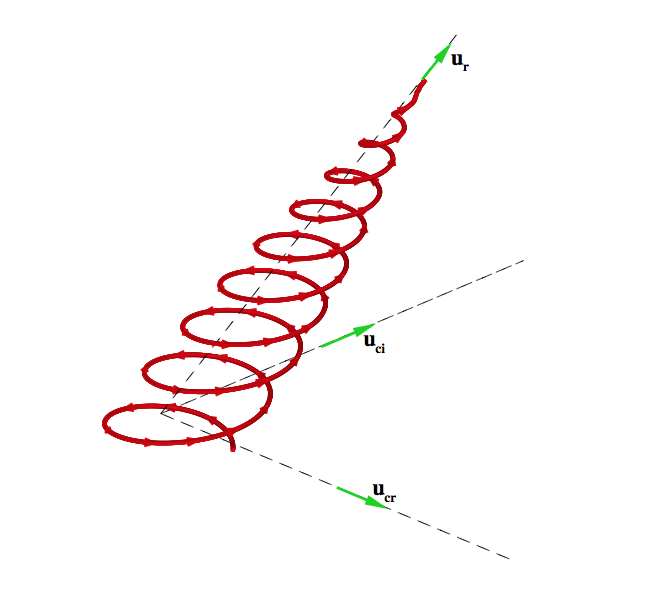
\includegraphics[clip=true, trim= 0.0cm 0.0cm 0.0cm 0.0cm,width=0.99\linewidth]{./figures/vorcord} 
\caption{Illustration of the vortex system \cite{mohamed2012eddy}.}
\end{figure}
%%%%%%%%%%%%%%%%%%%%%%%%%%%%%%%%%%%
The concept of the eddy-preserving limiter is to prevent the slope limiter to be activated (or to use a less dissipative limiter) during the reconstruction of the velocity component along the tangential direction of a vortex. To identify vortical flow regions, the enhanced swirling strength criterion of Chakraborty et al. \cite{chakraborty2005relationships} is employed, whereby in a vortical region, the velocity gradient tensor $\pmb\bigtriangledown\mathbf{v}$ possesses a conjugate pair of complex eigenvalues,
\begin{align} 
\sigma ( \pmb \bigtriangledown \mathbf{v})=  \left \{\lambda_{r}, \lambda_{cr}+i\lambda_{ci}, \lambda_{cr}-i\lambda_{ci} \right \}, \left |\lambda_{ci}\right | > \epsilon, \end{align}
where $\epsilon$ is a small positive real number. A local measure for the compactness of the vortical motion is added to further limit the vortical regions to areas where the following condition is satisfied,
\begin{align} 
-\zeta \leq \frac{\lambda_{cr}}{\lambda_{ci}}\leq \delta, \label{eq:1}
\end{align}
where $\zeta$ and $\delta$ are positive thresholds for verifying the compactness of the vortex. The velocity gradient tensor can be decomposed into the following form,
\begin{align} 
\pmb\bigtriangledown\mathbf{v}=\begin{bmatrix}
\hat{\mathbf{u}}_{r} & \hat{\mathbf{u}}_{cr} & \hat{\mathbf{u}}_{ci} 
\end{bmatrix}
\begin{bmatrix}
 \lambda_{r}&0&0 \\ 
 0&\lambda_{cr}&\lambda_{ci}\frac{\left |\mathbf{u}_{cr}\right |}{\left |\mathbf{u}_{ci}\right |}\\ 
 0&-\lambda_{ci}\frac{\left |\mathbf{u}_{ci}\right |}{\left |\mathbf{u}_{cr}\right |}&\lambda_{cr} 
\end{bmatrix}
\begin{bmatrix}
\hat{\mathbf{u}}_{r} & \hat{\mathbf{u}}_{cr} & \hat{\mathbf{u}}_{ci} 
\end{bmatrix}^{-1},
\end{align}
where $\hat{\mathbf{u}}_{r}$, $\hat{\mathbf{u}}_{cr}$, and $\hat{\mathbf{u}}_{ci}$ are normalized eigenvectors of the velocity gradient tensor.
%%%%%%%%%%%%%%%%%%%%%%%%%%%%%%%%%%%
The mapping and transformation matrix from the original Cartesian system $\mathbf{S}_{0}$ to the local vortex system $\mathbf{S}_{\omega}$ spanned by $\hat{\mathbf{u}}_{r}$, $\hat{\mathbf{u}}_{cr}$, and $\hat{\mathbf{u}}_{ci}$, are given by,
\begin{align} 
\begin{bmatrix}
\hat{\mathbf{M}}
\end{bmatrix}:\mathbf{S}_{0} \mapsto \mathbf{S}_{\omega}\; \; \; \; \; \begin{bmatrix}
\hat{\mathbf{M}}
\end{bmatrix}=\begin{bmatrix}
\hat{\mathbf{u}}_{r} & \hat{\mathbf{u}}_{cr} & \hat{\mathbf{u}}_{ci} 
\end{bmatrix}^{-1}.
\end{align}
The algorithm for the eddy-preserving limiting procedure is described below:
\renewcommand{\labelenumi}{\arabic{enumi}.}
\begin{enumerate}[nolistsep]

\item Calculate eigenvalues of the velocity gradient tensor $\pmb\bigtriangledown\mathbf{v}$. If the velocity gradient tensor has only real eigenvalues, then exit and employ the conventional van Albada limiter.

\item Verify the compactness of the vortical motion using Eqn.~\ref{eq:1}. If the flow lacks vortical compactness, then exit and employ the conventional van Albada limiter.

\item Calculate eigenvectors of the velocity gradient tensor $\pmb\bigtriangledown\mathbf{v}$, and define the transformation matrix $\begin{bmatrix}
\hat{\mathbf{M}}
\end{bmatrix}$. 

\item Transform velocity components into the vortex system $\mathbf{S}_{\omega}$.

\item In the axial direction, reconstruct variables using the conventional van Albada limiter with $\kappa=\frac{1}{3}$.

\item In the swirl plane, reconstruct variables using a higher $\kappa$ which leads to less artificial dissipation and inactivate the van Albada limiter by setting $\Phi_{i} = \Phi_{i+1} = 1$. 

\item Transform interpolated velocity components back to the original system $\mathbf{S}_{0}$ and evaluate the fluxes.

\end{enumerate}



